%!TEX root = ../template.tex
%%%%%%%%%%%%%%%%%%%%%%%%%%%%%%%%%%%%%%%%%%%%%%%%%%%%%%%%%%%%%%%%%%%
%% chapter1.tex
%% NOVA thesis document file
%%
%% Chapter with introduction
%%%%%%%%%%%%%%%%%%%%%%%%%%%%%%%%%%%%%%%%%%%%%%%%%%%%%%%%%%%%%%%%%%%

\typeout{NT FILE chapter1.tex}%

\chapter{X-ray Tracing}
\label{cha:xray_tracing}

\par X-ray imaging is a critical diagnostic tool used by medical professionals to diagnose and treat various illnesses and injuries. While the use of x-rays is essential to provide immediate, life-saving results, the amount of radiation dosage patients receive can be more than medically necessary. This excessive radiation exposure can increase the risk of cancer and other potential health risks, making it crucial to minimize the amount of radiation exposure patients receive during x-ray imaging \cite{RadiationEffects}.

\par While one could minimize radiation dosage by adding shielding and/or changing the position of the target/x-ray source and obtain a reported dosage from the x-ray machine software, this approach has limitations. First, it is time-consuming in often urgent situations, and it still does not guarantee the optimal imaging parameters. Secondly, when it comes to resource-limited settings, the increased cost of imaging procedures due to this optimization procedure may not be financially viable.

\par In addition to minimizing dosage, it's equally important to accurately quantify and record the amount of dosage a patient receives over time, for it is the cumulative dose which poses the greatest threat \cite{lauer2009elements}. Typically, exposure is measured using absorbed dose in the body and air kerma at the skin layer, which both have units of grays (joule/kg), making it directly related to the energy deposited by photons and their secondary particles. Often, these values are estimated based on the properties of the x-ray source and the specific procedure being performed. However, these are typically very rough estimates, thus necessitating a physics-based model that can accurately simulate the traversal of x-rays through a medium and calculate the associated dosage.

\par To address these challenges, a research project focusing on the development and validation of a computational modeling approach for x-ray attenuation and medical imaging simulation using ray tracing was initially proposed. The goal of this approach was to accurately simulate the image one might obtain from an x-ray machine, while also estimating the associated dosage. This approach to x-ray simulation used ray tracing, a common graphics technique that simulates particles of light traveling in a 3D environment. In this environment, one could place models of objects and trace the path of photons through them. By using the objects' attenuation coefficient, which describes how strongly a material weakens or reduces the strength of x-rays as they pass through, and the distance light travels through the object, it was proposed that one would be able to calculate the attenuation of the x-ray and simulate the expected x-ray image.

\section{Ray Tracing}
\par Ray tracing is a computer graphics technique that involves tracing the path of rays as they pass through a virtual scene. Due to its ability to create highly-realistic images, ray tracing has been used extensively in animations, video games, scientific computing, and by designers who need a physically accurate design of a product. While not the only rendering technique or the fastest in computer graphics, its ability to consistently produce physically realistic renders has made it an indispensable tool in many industries. By accurately simulating the behavior of light, ray tracing can capture intricate details of how light interacts with objects, resulting in realistic shadows, reflections, refractions, and global illumination effects. This level of visual fidelity allows for the creation of visually stunning and immersive experiences that were previously challenging to achieve. As hardware capabilities continue to advance and real-time ray tracing becomes more accessible, its applications are expanding, and its impact on various fields is growing, pushing the boundaries of what is possible in computer graphics and visual simulation \cite{Peddie}.

\section{The Brute Force Algorithm}
The rays in a scene are described mathematically as the parametric representation of a line. In three dimensions, the point at the end of the line $\va*{r}$ at parameter $t$ is given by the following equation:

\begin{equation}
\va*{r}(t) = \va*{r_0} + \vu*{d} t,
\label{eq:parametric_ray}
\end{equation}

\noindent where $\va*{r_0}$ points from the origin to the start of the line and $\vu*{d}$ is a unit vector parallel to the direction of the line. The described ray is shown in Figure~\ref{fig:ray_diagram}.\\

\begin{figure}[H]
    \centering
	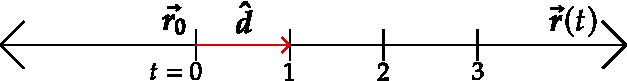
\includegraphics[width=\textwidth]{chapter1/RayDiagram.pdf}
	\caption{A diagram of a parametric ray.}
	\label{fig:ray_diagram}
\end{figure}

\par Unlike in real life where light rays end at a camera, we instead trace light rays from the camera to locations in the scene. While one could trace light rays from a light source (forward ray tracing), many of these rays would end up missing the camera entirely, not affecting the image. More efficiently, the light rays are instead traced from the camera to the light source (backward ray tracing), drastically cutting back on the computational load while producing an identical image for most practical cases \cite{Peddie}. So, in the case of backward ray tracing, the method used in this research, rays are emitted from the camera; therefore, $\va*{r_0}$ represents the location of the camera in the scene.

\par To define the area of the scene visible from the point of view of the camera, one can create a rectangular surface in which all rays pass through, called a viewport. Increasing the size of the viewport increases the amount of the scene that is visible in the final image, and vice versa. This viewport is broken up into a grid, the resolution of which determines the resolution of the final image. Rays are then sent through each point in this grid and out into the scene.

\par So far, we have a camera, light rays, and a way to define what parts of the scene are visible; all three of which are visualized in Figure~\ref{fig:basic_ray_tracing_setup}. It is important to note that, by convention, the $z$-axis in the scene points opposite the viewport.

\begin{figure}[H]
  \centering
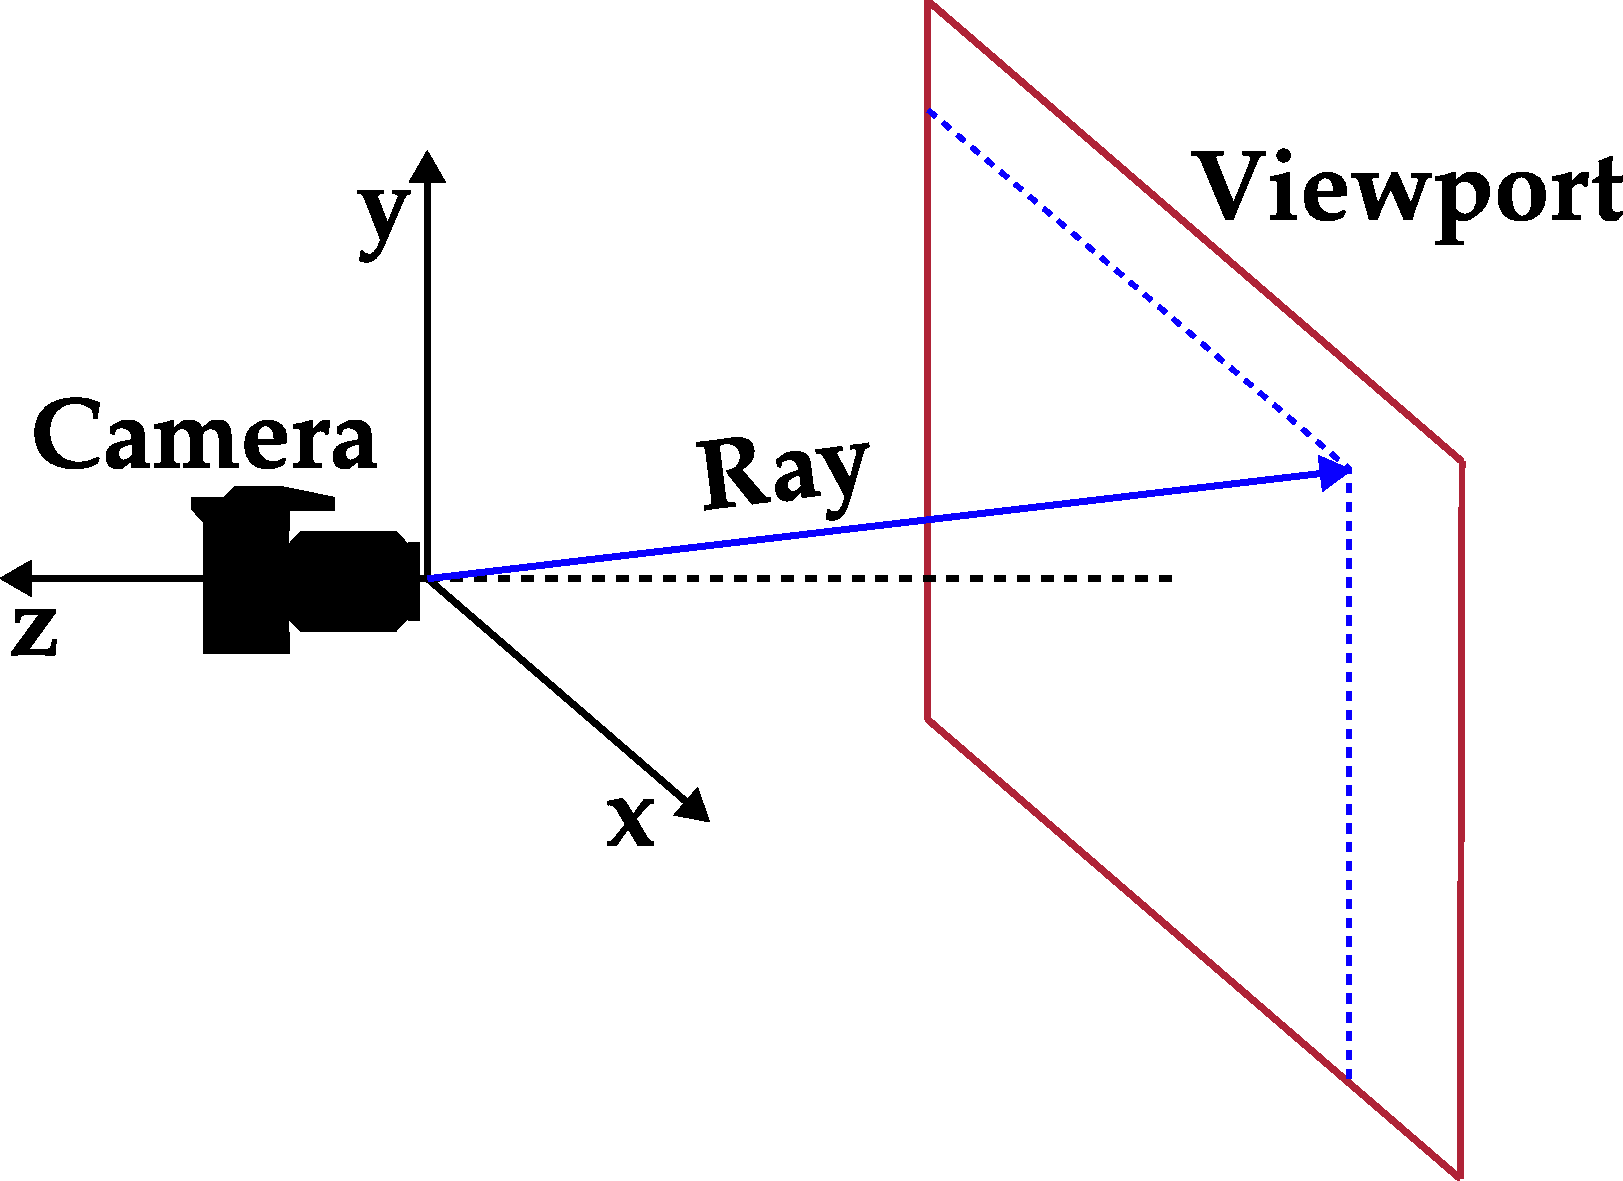
\includegraphics[width=\textwidth]{chapter1/RayTracingSetup.pdf}
\caption{A basic ray-tracing setup with a camera, ray, and viewport.}
\label{fig:basic_ray_tracing_setup}
\end{figure}

\par To set the location of the viewport in the scene, we must first define three new vectors: $\val{HO}$, $\val{VE}$, and $\val{FL}$, which are vectors pointing from the left most to right most point (-$x$ to $x$ direction), the bottom most to top most point (-$y$ to $y$ direction), and from the center of the viewport to $\va*{r_0}$, respectively. A vector pointing from $\va*{r_0}$ to the bottom-left corner $\val{LHC}$ can be calculated using the following equation:

\begin{equation}
  \val{LHC} = \va*{r_0} - \frac{1}{2}\val{HO} - \frac{1}{2}\val{VE} - \val{FL},
  \label{eq:LHC}
\end{equation}

\noindent which was obtained geometrically from Figure~\ref{fig:LHC_diagram} \cite{Shirley}.

\begin{figure}[H]
    \centering
	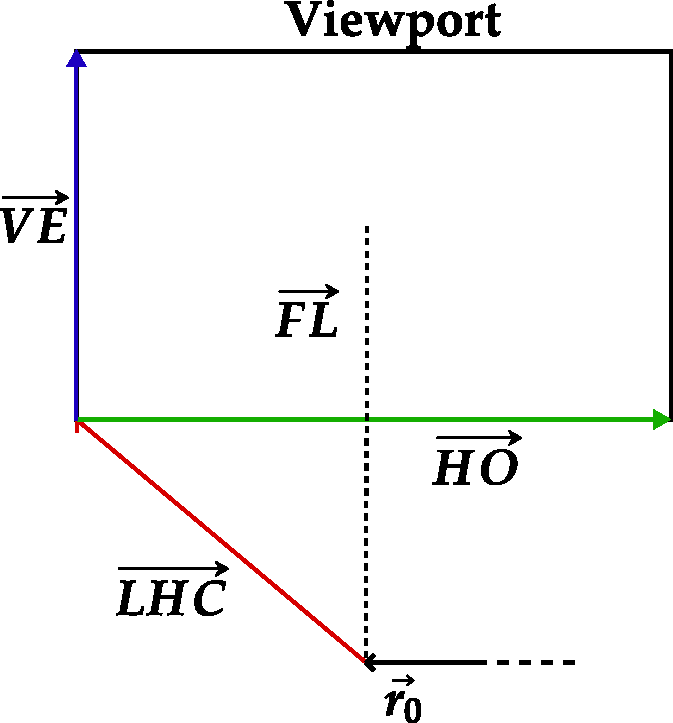
\includegraphics[width = 0.8\textwidth]{chapter1/LHCDiagram.pdf}
	\caption{A diagram showing the geometric representations of $\protect\val{HO}$, $\protect\val{VE}$,
   $\protect\val{FL}$, and $\protect\val{LHC}$ with respect to the viewport.}
	\label{fig:LHC_diagram}
\end{figure}

\par With $\val{LHC}$ pointing to the left-hand-corner of the viewport in the scene, $\val{HO}$ and $\val{VE}$ can be scaled to define a ray pointing from the camera to any point on the viewport. In particular,  the viewport's horizontal and vertical coordinates, $u_i$ and $v_j$, are defined as such,

\begin{align}
u_i &= i/(\text{image width} - 1);\\
v_j &= j/(\text{image height} - 1),
\label{eq:viewport_coords}
\end{align}

\noindent where the image width and height are the resolution of the rendered image, $i$ is an integer ranging from [0, image width - 1], and $j$ is an integer ranging from [0, image height - 1]. Note that both $u_i$ and $v_j$ range from [0, 1].

\par Therefore, using these newly defined viewport coordinates, a ray taking the form of Equation~\ref{eq:parametric_ray}, pointing from the camera to the pixel coordinates $(i, j)$ is given by the following equation:

\begin{equation}
  \va*{r}_{\bm{i,j}}(t) = \va*{r_0} + t \left( \val{LHC} + u_i \val{HO}  + v_j \val{VE} \right),
  \label{eq:ray_to_viewport}
\end{equation}

\noindent which is represented geometrically in Figure~\ref{fig:ray_to_viewport_diagram} \cite{Shirley}.

\begin{figure}[H]
  \centering
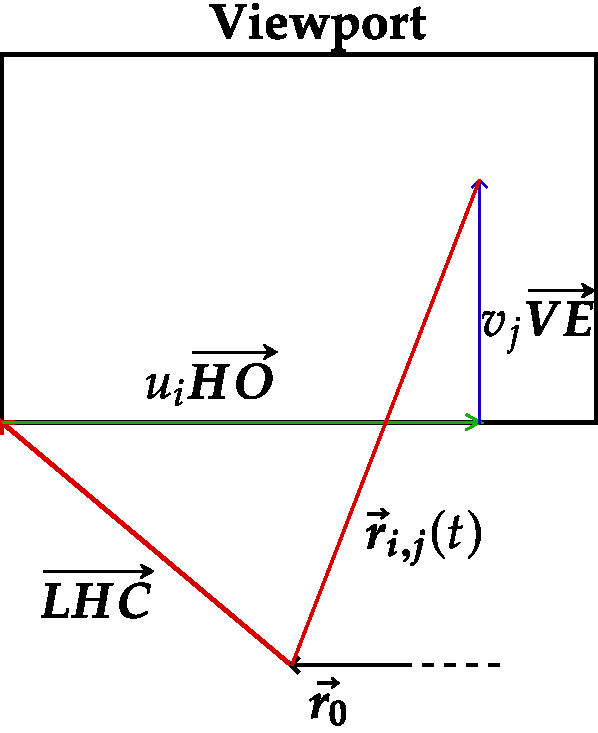
\includegraphics[width = 0.7\textwidth]{chapter1/RayToViewportDiagram.pdf}
\caption{A diagram showing the geometric representation of Equation~\ref{eq:ray_to_viewport}.}
\label{fig:ray_to_viewport_diagram}
\end{figure}

\section{Ray-Triangle Intersections}
\par With the end goal to be able to ray-trace x-rays through an arbitrary user-defined mesh, we first need to choose which shape to compose said mesh with. Due to its efficient ray-intersection algorithm and its ease of parallelization on Graphics Processing Units (GPUs), these constituents, referred to as primitives, are typically chosen to be triangles. The following section will develop the ray-triangle intersection algorithm used by the x-ray tracer. In particular, the algorithm used was invented by Tomas Möller and Ben Trumbor, and is subsequentially refered to as the Möller-Trumbore ray-triangle intersection algorithm \cite{moller2005fast}. 

\subsection{Barycentric Coordinates}
\par To motivate the unique coordinate system used by the algorithm, let us first review the concept of center of mass for 3 massive point particles. If 3 objects each have their own location in space $\va*{r_i}$, each with mass $m_i$, the center of mass $\va*{R}$ is given by:

\begin{equation}
  \va*{R} = \frac{m_1 \va*{r_1} + m_2 \va*{r_2} + m_3 \va*{r_3}}{m_1 + m_2 + m_3}.
  \label{eq:com}
\end{equation}

Notice a few properties of $\va*{R}$ that are intuitively clear:

\begin{itemize}
\item $\va*{R}$ will always lie in the plane containing the point particles.
\item $\va*{R}$ will always lie in the triangle $T$ with vertices \{$\va*{r_i}$\}.
\end{itemize}

\noindent This means that by changing \{$m_i$\}, $\va*{R}$ will span all set of points in T. This is the motivation behind barycentric coordinates, the coordinate system employed by Möller and Trumbore. In particular, to represent a vector $\va*{v}$ pointing to the surface of a triangle $T \in \mathbb{R}^3$ with vertices $\va*{v_0}$, $\va*{v_1}$, and $\va*{v_2}$, barycentric coordinates can be utilized. These coordinates \{$\alpha, \beta, \gamma\}\in \mathbb{R}$ act as the masses of the vertices of $T$. Thus, any point $\va*{v}$ along the plane $P$ of $T$ can be represented by 

\begin{equation}
\va*{v} = \alpha \va*{v_0} + \beta \va*{v_1} + \gamma \va*{v_2}.
\label{eq:v_on_plane_bary}
\end{equation}

\noindent For $\va*{v}$ to be located on or within $T$, the following requirements on the barycentric coordinates must be satisified:

\begin{align}
  &\text{\textbullet}\quad \alpha + \beta + \gamma = 1 \label{eq:sum_to_1_bary}\\
  &\text{\textbullet}\quad \alpha, \beta, \gamma \geq 0 \label{eq:greater_than_0_bary}
\end{align}

With regard to the center of mass interpretation, Equation~\ref{eq:sum_to_1_bary} removes the computation of the denominator in Equation~\ref{eq:com}, while Equation~\ref{eq:greater_than_0_bary} eliminates the possibility of negative mass. For a rigorous proof of the requirements, see \cite{capitan2015barycentric}.

\subsection{Möller-Trumbore Intersection Algorithm} \label{sec:ray_tri_alg}
\par The algorithm consists of 2 main steps:

\begin{enumerate}
  \item Check if ray intersects with $P$;
  \item If so, check if intersection lies outside of $T$.
\end{enumerate}

\subparagraph{1.}
\par To check if the ray described by Equation~\ref{eq:parametric_ray} intersects with $P$, one can define two vectors that lie along 2 edges of $T$:

\begin{align}
  \va*{e_1} &= \va*{v_1} - \va*{v_0} \label{eq:e_1_bary};\\
  \va*{e_2} &= \va*{v_2} - \va*{v_0} \label{eq:e_2_bary}.
\end{align}

\noindent If $\va*{p} = \vu*{d} \cross \va*{e_2}$, then let $C = \va*{e_1} \cdot \va*{p}$. The line $\va*{r}$ does not intersect the plane $P$ iff $C = 0$, which happens iff $\vu*{d} \parallel P$. Thus, if $C = 0$, then $\va*{r}$ does not intersect $P$; otherwise, $\va*{r}$ will intersect $P$.

\subparagraph{2.}
Solving Equation~\ref{eq:sum_to_1_bary} for $\alpha$ and substituting into Equation~\ref{eq:v_on_plane_bary} results in

\begin{equation}
 \va*{v} = (1 - \beta - \gamma)\va*{v_0} + \beta\va*{v_1} + \gamma\va*{v_2}.
 \label{eq:r_no_alpha_bary}
\end{equation}

\noindent After distributing and rewriting Equation~\ref{eq:r_no_alpha_bary} in terms of $\va*{e_1}$ and $\va*{e_2}$, 

\begin{equation}
  \va*{v} = \va*{v_0} + \beta \va*{e_1} + \gamma \va*{e_2}.
  \label{eq:r_no_alpha_bary_simp}
\end{equation}

\noindent Setting $\va*{r} = \va*{v}$ to find the barycentric coordinates for the ray-triangle intersection and solving for $\va*{r_0} - \va*{v_0}$ yields

\begin{equation}
  \va*{r_0} - \va*{v_0} = -\vu*{d}t + \beta \va*{e_1} + \gamma \va*{e_2}.
\end{equation}

\noindent One can then show that taking $(\va*{r_0} - \va*{v_0}) \vdot \va*{p}$ gives the following equation for $\beta$:

\begin{equation}
  \beta = \frac{(\va*{r_0} - \va*{v_0}) \vdot \va*{p}}{C},
  \label{eq:beta_bary}
\end{equation}

\noindent and similarly, taking $\vu*{d} \vdot [(\va*{r_0} - \va*{v_0}) \cross \va*{e_1}]$ results in

\begin{equation}
  \gamma = \frac{\vu*{d} \vdot [(\va*{r_0} - \va*{v_0}) \cross \va*{e_1}]}{C}.
  \label{eq:gamma_bary}
\end{equation}

\noindent To then determine $t$ at which the ray-triangle intersection occurs, one can take $\va*{e_2} \vdot [(\va*{r_0} - \va*{v_0}) \cross \va*{e_1}]$, yielding

\begin{equation}
  t = \frac{\va*{e_2} \vdot [(\va*{r_0} - \va*{v_0}) \cross \va*{e_1}]}{C}.
  \label{eq:t_bary}
\end{equation}

\noindent Since Equation~\ref{eq:sum_to_1_bary} is assumed upon the construction of Equation~\ref{eq:r_no_alpha_bary}, one only needs to verify that Equation~\ref{eq:greater_than_0_bary} is satisfied to determine if there is a ray-triangle intersection. In addition, since certain scenarios might require a finite length ray described by $t\in[t_{\textrm{min}}, t_{\textrm{max}}]$, one would also check if the $t$ of the intersection falls within this range. The implementation of this algorithm used in the C++ x-ray tracing code is shown in Listing~\ref{lst:tri_intersect_alg}.

\begin{listing}
\begin{minted}[linenos]{cpp}
  bool triangle::hit(const ray &r, float t_min, float t_max, hit_record &rec) const {
    float kEpsilon = 1e-9;

    vec3 e1 = v1 - v0;
    vec3 e2 = v2 - v0;
    vec3 pvec = cross(r.direction(), e2);
    float C = dot(e1, pvec);

    // ray is parallel to triangle
    if (std::abs(C) < kEpsilon) return false; 

    float inv_C = 1.0 / C;

    vec3 tvec = r.origin() - v0;
    float beta = dot(tvec, pvec) * inv_C;

    // hit point is outside of triangle
    // if beta > 1.0 -> alpha and/or beta < 0
    if (beta < 0.0 || beta > 1.0) return false;

    vec3 qvec = cross(tvec, e1);
    float gamma = dot(r.direction(), qvec) * inv_C;

    // hit point is outside of triangle
    // if beta + gamma > 1.0 -> alpha < 0
    if (gamma < 0.0 || beta + gamma > 1.0) return false;

    float t = dot(e2, qvec) * inv_C;

    // hit point is outside of ray's range
    if (t < t_min || t > t_max) return false;

    // record intersection point
    rec.t.push_back(t); 
    rec.p.push_back(r.at(t));

    return true;
}
\end{minted}
\caption{C++ implementation of the Möller-Trumbore ray-triangle intersection algorithm.}
\label{lst:tri_intersect_alg}
\end{listing}

\section{Meshes and Their Intersections}
From these triangle primitives, one can easily construct a mesh. In particular, one can create an STL file, which is a list of triangles with each element containing the vertices and unit normal vector of a particular triangle. These files, which must describe closed meshes, can then be specified in the x-ray tracing code, along with their position in the scene and their composing material $M$. An example STL mesh is shown in Figure~\ref{fig:coin_mesh_render}.

\begin{figure}[htb!]
  \centering
  \begin{subfigure}[b]{0.45\textwidth}
      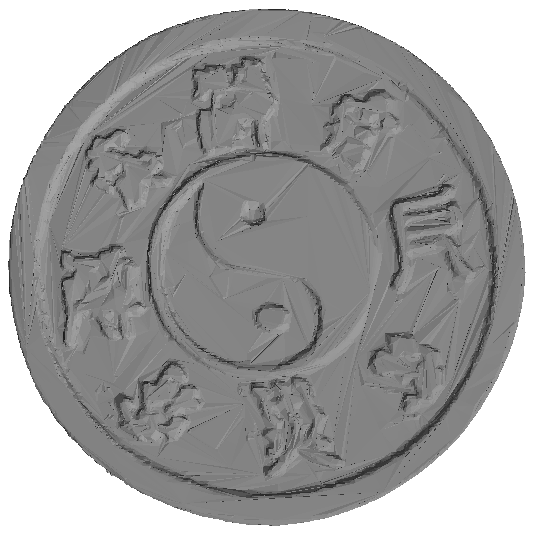
\includegraphics[width=\textwidth]{chapter1/coin_top.png}
      \caption{Top}
  \end{subfigure}
  \hfill % optional spacing
  \begin{subfigure}[b]{0.45\textwidth}
      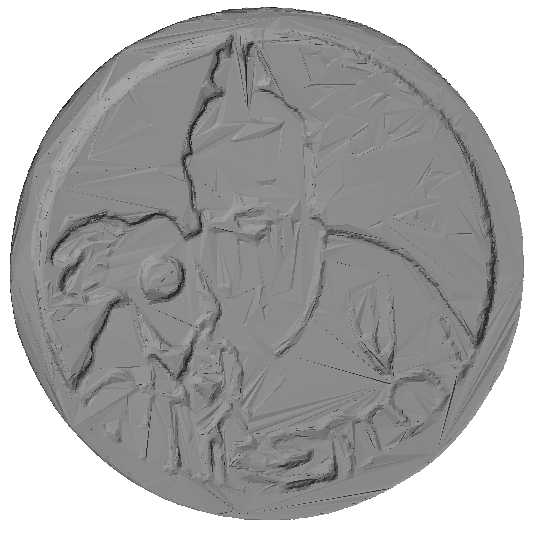
\includegraphics[width=\textwidth]{chapter1/coin_bottom.png}
      \caption{Bottom}
  \end{subfigure}
  \caption{The rendered (a) top and (b) bottom of an STL mesh representing an ancient Chinese coin. This particular mesh is composed of 33,558 triangles.}
  \label{fig:coin_mesh_render}
\end{figure}

The key quantity of interest for an x-ray traversing through one of these meshes $S$ is the total length $l$ of the ray that exists within the mesh. To calculate $l$, the x-ray tracing code

\begin{enumerate}
  \item Loops through each triangle $T_i$ in $S$ and checks for an intersection using the Möller-Trumbore algorithm described in Section~\ref{sec:ray_tri_alg}. If the ray does not intersect with any $T_i$, then the ray is said to not intersect $S$ and $l=0$.
  \item If the ray intersects $N$ times with $S$, then the parameters $t_i$ of the intersected $T_i$'s are sorted in ascending order. 
  \item Since a ray can only enter then exit a mesh, 
  \begin{equation}
    l = \sum_{i=0}^{\frac{N-1}{2}} (t_{2i+1} - t_{2i}).
    \label{eq:l_for_M}
  \end{equation}
\end{enumerate}

\section{Intensity Drop}
With $l$ obtained from Equation~\ref{eq:l_for_M}, one can then calculate the effect on the ray's intensity $I$ after traversing $S$ using the exponential attenuation law developed in the typical undergraduate modern physics course \cite{serway}:

\begin{equation}
  I = I_0 e^{-\mu_m(M, E) \rho l},
  \label{eq:exp_atten}
\end{equation}

\noindent where $I_0$ is initial intensity of the ray before entering $S$, $\mu_m(M, E)$ is the mass-attenuation coefficient of the material $M$ composing $S$ at energy $E$, and $\rho$ is the mass density of $M$. 

\par Furthermore, if one considers a single photon travelling a distance $l$ through $S$, the ratio $\frac{I}{I_0}$ would represent the probability of completing the traversal. Thus, one can use the multiplication rule of probabilities to generalize Equation~\ref{eq:exp_atten} to find the relative intensity $\frac{I_k}{I_0}$ of a ray after traversing a $k$ number of different $S$'s. In particular,

\begin{equation}
  \frac{I_k}{I_0} = \prod_i^{k} \frac{I_i}{I_0} =  \exp\left[ -\sum_i^k \mu_m(M_i, E) \rho_i l_i \right],
  \label{eq:exp_atten_k}
\end{equation}

\noindent where $M_i$, $\rho_i$, and $l_i$ is the material, mass density, and path length, respectively, of the $i$-th traversed $S$.

\par Recall that these rays are being sent out from a source (camera) to a grid of points of a specified resolution (viewport). In the case of x-ray imaging, the camera would represent the x-ray tube, while the viewport would be the x-ray detector. So, these meshes would be placed between the tube and detector, and rays would lose intensity in their path from the tube to the detector, revealing details of the meshes' geometries and compositions. In order to visualize these variations in intensities, the x-ray tracing code directly converts the relative intensity values into pixels of an 8-bit grayscale image. These relative intensities obtained from Equation~\ref{eq:exp_atten_k} are converted to integers in the range of 0 to 255, where $\frac{I_k}{I_0}$'s of 1 would become 255 (white pixel), and values of 0 would stay 0 (black pixel). It is important to note the versatility in image interpretation: the inversion of image color, a practice variable across different X-ray machines, does not compromise the information contained. This manipulation, sometimes employed by radiologists for enhanced detail visibility, alters none of the underlying data. Rather, it serves to accentuate certain details, making them more discernible visually. Moreover, advanced imaging software often allows radiologists to adjust the contrast and brightness of x-ray images post-processing, further aiding in the identification and analysis of specific features or anomalies within the image.


\par For a flowchart summarizing the x-ray tracing algorithm introduced in this chapter, see Figure~\ref{fig:xray_trace_flowchart}.
\newpage
\begin{figure}[htb!]
  \centering
  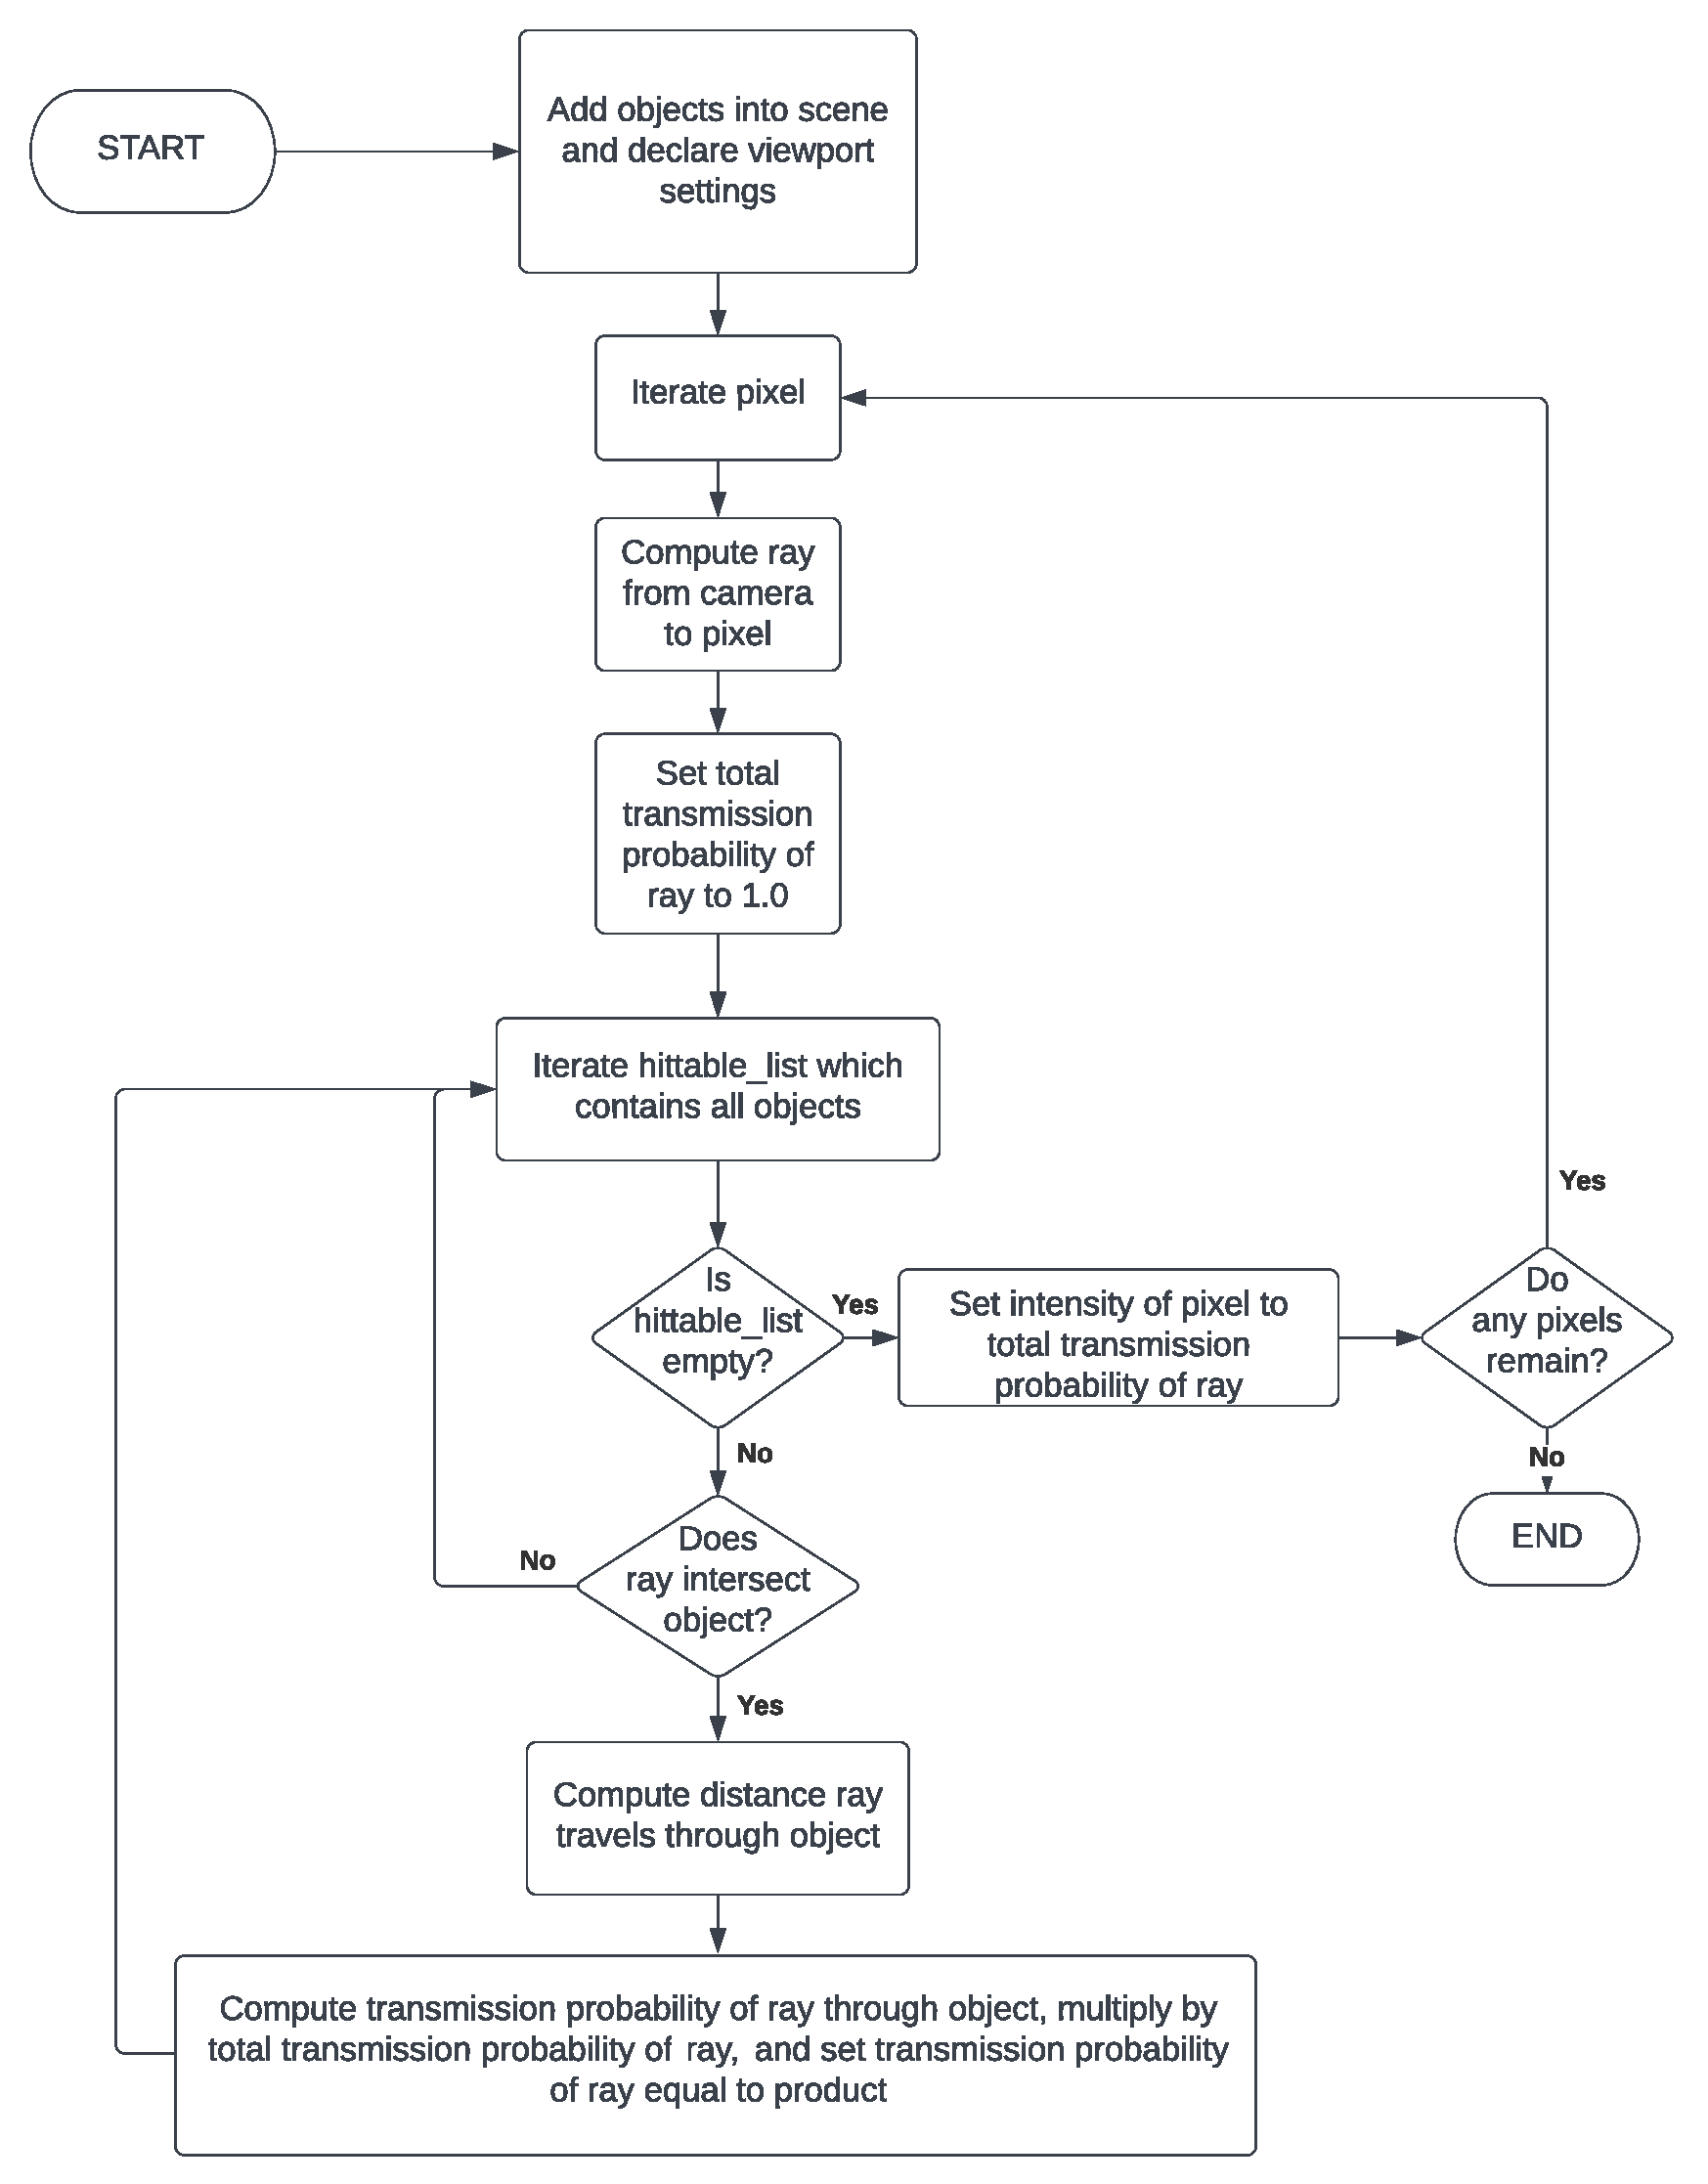
\includegraphics[width=\textwidth]{chapter1/X-RayTracingAlgorithmFlowChart.pdf}
  \caption{A flowchart summarizing the x-ray tracing algorithm introduced in Chapter~\ref{cha:xray_tracing}.}
  \label{fig:xray_trace_flowchart}
\end{figure}
\newpage
\section{Mass-Attenuation Coefficients and Material Definition Sources}
In practice, one needs a source of the $\mu_m$'s used in Equation~\ref{eq:exp_atten_k}. The source of these values used by the x-ray tracing code is NIST's tables of x-ray mass-attenuation coefficients obtained by Hubbell \cite{hubbell1982photon}. These tables are given for each element $Z$, from which we can approximate $\mu_m$ of a material $M$ by taking the weighted average of the mass fractions of its constituent elements and their respective $\mu_m$'s. In particular, the mass-attenuation coefficient of a particular $M$ at $E$, composed of elements ${Z_i}$ with mass fractions ${w_i}$, is given by

\begin{equation}
  \mu_m(M, E) = \sum_i w_i \mu_m(Z_i, E),
  \label{eq:mu_weighted}
\end{equation}

\noindent with {$Z_i$} and {$w_i$} of common materials provided by NIST \cite{hubbell1982photon}.

\section{Example Renders}
With the x-ray tracing theory and methodology developed, it was then implemented in the programming language C++. For details on this implementation, see the source code in its GitHub repository \cite{xraytracing_git}. Located in Figure~\ref{fig:example_renders} are examples of x-ray images rendered using the program.

\begin{figure}[htb!]
  \centering
  \begin{subfigure}[b]{\textwidth}
    \centering
    
\includegraphics[width=0.28\textwidth]{chapter1/coin.png}
    \caption{Ancient Chinese Coin (shown in Figure~\ref{fig:coin_mesh_render}): $M =$ Bone, $E = \qty{30}{keV}$}
  \end{subfigure}
  \\[1ex]
  \begin{subfigure}[b]{0.45\textwidth}
    \centering
      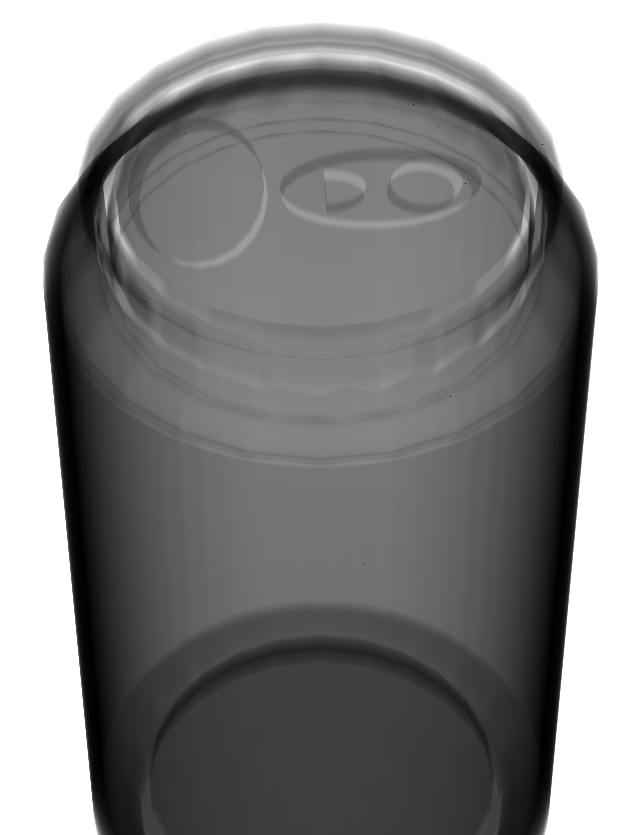
\includegraphics[width=0.45\textwidth]{chapter1/sodaCan.png}
      \caption{Soda Can: $M =$ Aluminum, $E = \qty{40}{keV}$}
  \end{subfigure}
  \hfill % optional spacing
  \begin{subfigure}[b]{0.45\textwidth}
      \centering
      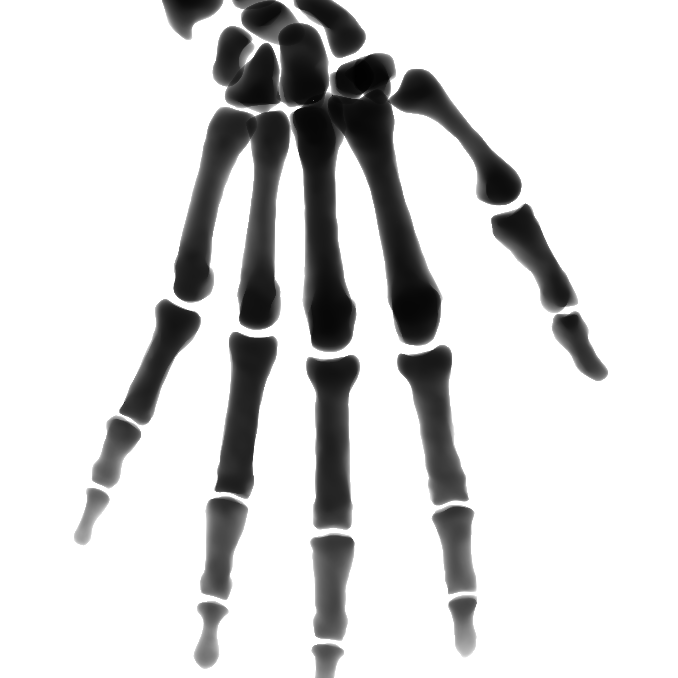
\includegraphics[width=0.55\textwidth]{chapter1/anatomicallyCorrectHand.png}
      \caption{Human Hand: $M =$ Bone, $E = \qty{40}{keV}$}
  \end{subfigure}
  \caption{A few example x-ray images rendered using the x-ray tracing code.}
  \label{fig:example_renders}
\end{figure}







  






